%==============================================================================
% Šablona prezentace/Presentation template
% Autoři / Authors: Zdeněk Vašíček, Aleš Smrčka, Jaroslav Dytrych, Jana Stopková, Kristýna Zaklová, Adam Herout
% Kontakt pro dotazy a připomínky: sablona@fit.vutbr.cz
% Contact for questions and comments: sablona@fit.vutbr.cz
%==============================================================================

\documentclass[]{fitthesispresn}

\usepackage[czech, ruled, linesnumbered]{algorithm2e}
\usepackage{algorithmicx}

% Nastavení informací pro úvodní stránku / Setting information for the title page
%---------------------------------------------------------------------------
\projectinfo{
  date=\today, % Datum - je vhodné vepsat datum obhajoby (natvrdo), ne datum kompilace slajdů / Date - it is advisable to write the date of the defense (hard), not the date of the slide compilation        
  title={Cyklická fronta}, % Název prezentace / Presentation title (The whole title of the presented work suitably divided into lines that are optically balanced)
  title.footer={Cyklická fronta}, % Název prezentace - text zobrazovaný vedle čísla slajdu / Presentation title - displayed next to the slide number (The full title of the presented work, it may be suitably abbreviated to fit the footer)
  author.name={Lukáš},  % Jméno autora / Author name
  author.surname={Pšeja}, % Příjmení autora / Author surname
  author.title.first={} % Tituly před jménem autora (jsou-li jaké) / Author's titles before the name (if there are any)
}

% Struktura prezentace / Presentation structure
%---------------------------------------------------------------------------

\begin{document}
    \frame[plain]{\titlepage} % Úvodní stránka / Title page

    \begin{frame}
        \frametitle{Motivace}
        \begin{itemize}
            \item Cyklická fronta se často využívá v praxi
            \item Je využívána v plánovačích procesů operačních systémů, v síťových systémech při řízení front datových packetů a celkově v systémech, kde je potřeba periodicky zpracovávat události nebo data
            \item \emph{Výhody}\,--\,rychlost, efektivita paměti, využití pro vyrovnávací paměť
            \item \emph{Nevýhody}\,--\,omezená velikost
        \end{itemize}
    \end{frame}

    \begin{frame}
        \frametitle{Co je to cyklická fronta?}
        \begin{columns}
            \column{0.5\textwidth}
            \begin{itemize}
                \item Cyklická fronta je \emph{datová struktura} pro ukládání dat
                \item Je implementovaná jako \emph{zacyklené pole}, což umožňuje \emph{nekonečný} pohyb v poli
                \item Ke správě slouží dva ukazatele, \emph{write} a \emph{read}
                \item Oproti lineárnímu poli je výhodou, že se \emph{nemusí} přesouvat prvky, ale pouze posouvají ukazatele
            \end{itemize}
            \column{0.5\textwidth}
            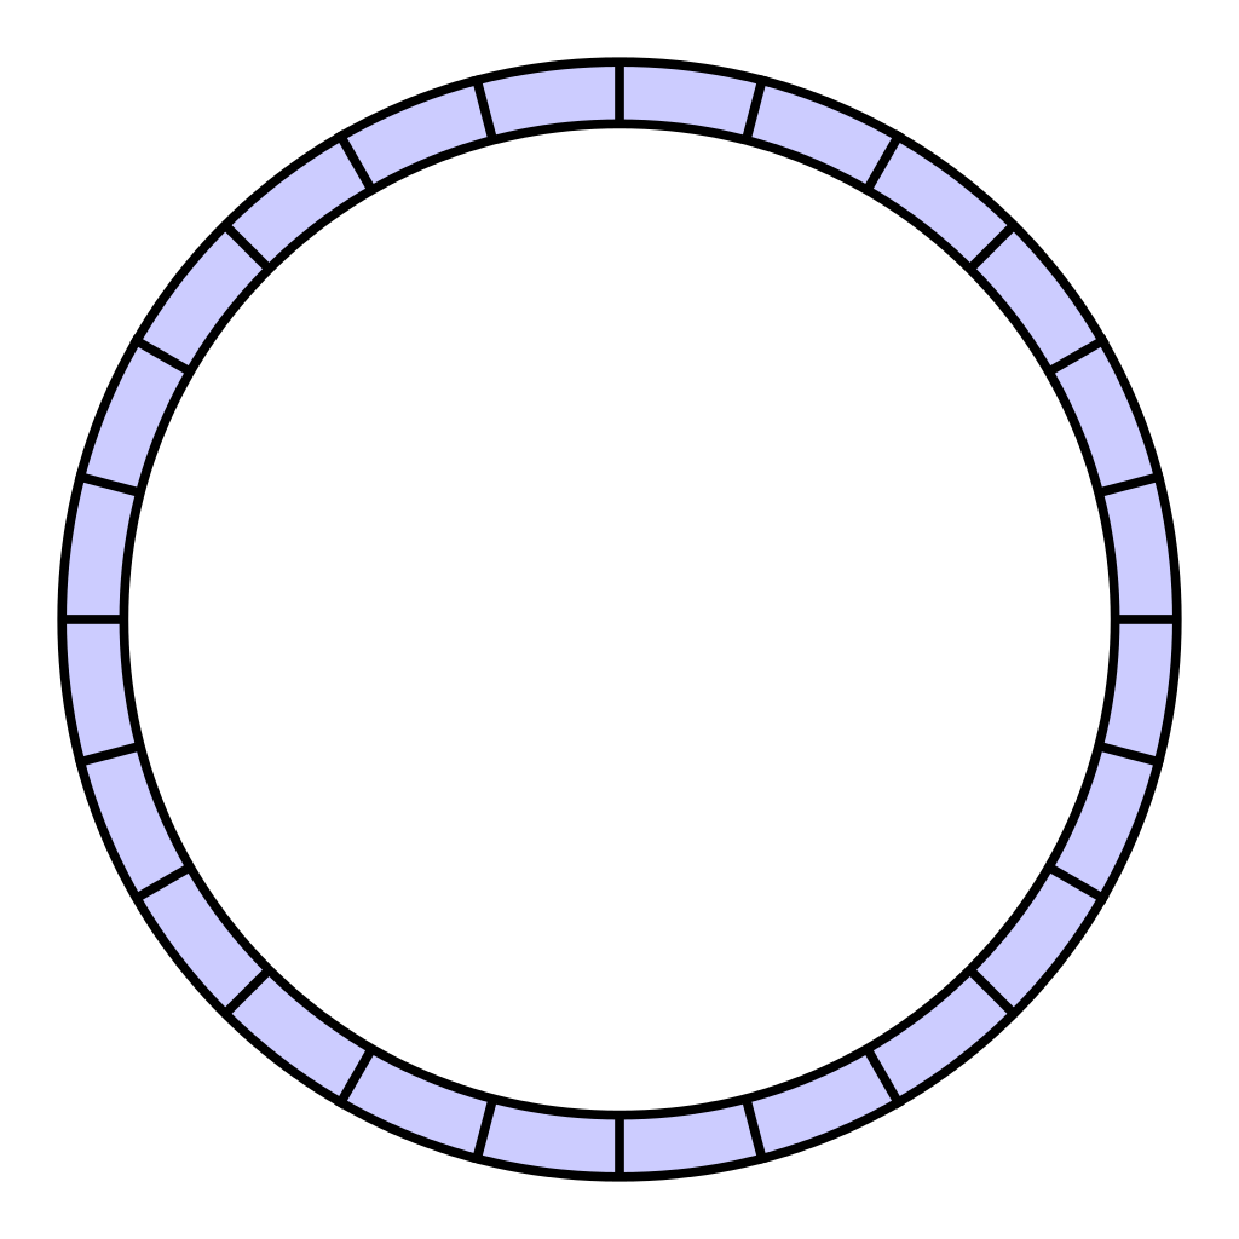
\includegraphics[width=\textwidth]{img/circular_buffer_empty_circle.pdf} % wikipedie - circular buffer
        \end{columns}
    \end{frame}

    \begin{frame}
        \frametitle{Struktura cyklické fronty}
        Při implementaci uvažujeme dva způsoby
        \begin{itemize}
            \item Jednodušší způsob, kdy používáme jeden záznam navíc, který nám říká, kolik je momentálně prvků v poli
            \item Složitější ale efektivnější způsob, kdy používáme ukazatele \emph{write} a \emph{read} na výpočet prvků v poli
        \end{itemize}
        Druhý způsob je výhodnější, protože je vhodný pro \emph{multithreading} a \emph{real-time} aplikace. Budeme implementovat UNIXovou funkci \emph{tail}
        \begin{algorithm}[H]
        \caption{CircularBuffer Structure}
        \label{alg:circularbuffer}
        \begin{algorithmic}[1]
            \State \textbf{Structure:} CircularBuffer
            \State \textbf{Fields:}
            \State \hspace{\algorithmicindent} $\bullet$ \textit{size} : Integer
            \State \hspace{\algorithmicindent} $\bullet$ \textit{head} : Integer
            \State \hspace{\algorithmicindent} $\bullet$ \textit{tail} : Integer
            \State \hspace{\algorithmicindent} $\bullet$ \textit{lines} : Pointer to Pointer to Character
        \end{algorithmic}
        \end{algorithm}
    \end{frame}

    \begin{frame}
        \frametitle{Zakladní operace s cyklickým polem}
        Kontrola prázdnosti a plnosti cyklického pole
    \end{frame}




    \begin{frame}
        \frametitle{Cíle práce}
        \begin{columns}
            \column{0.4\textwidth}
            \begin{itemize}
                \item \emph{Vstup}
                \item \emph{Výstup}
                \item Žádoucí \emph{vlastnosti}
                \item Využití \& aplikace
            \end{itemize}

            \column{0.6\textwidth}
            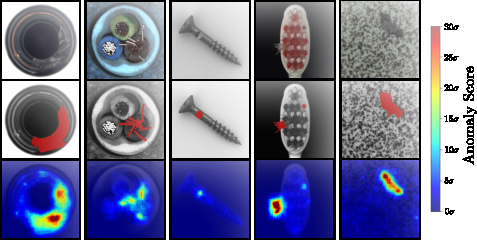
\includegraphics[width=\textwidth]{img/template-Goal.pdf}
        \end{columns}
    \end{frame}

    \begin{frame}
        \frametitle{Podstatné informace o řešení}
        \centering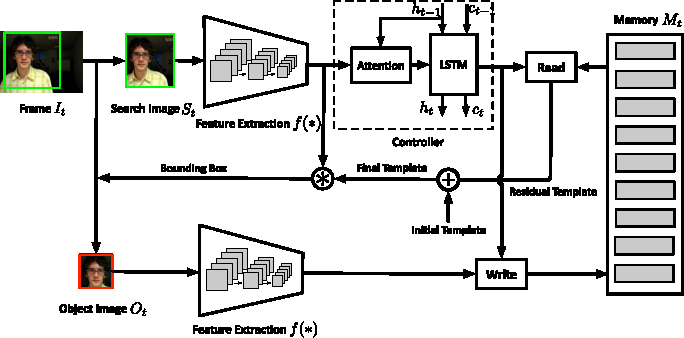
\includegraphics[width=0.8\textwidth]{img/template-Schema.pdf}
        \begin{equation}
            \mathbf{a}_t = \sum_{i=1}^{L}\alpha_{t,i}\mathbf{f}_{t,i}^{*}
        \end{equation}
        kde $\alpha_{t,i}$ počítá \emph{softmax}:
        \begin{align}
            \alpha_{t,i} & = \frac{\exp(r_{t,i})}{\sum_{k=1}{L}\exp(r_{t,k})}
            \\
            r_{t,i}      & = W^a \tanh\left( W^h \mathbf{h}_{t-1} + W^f\mathbf{f}_{t,i}^{*} + b \right)
        \end{align}
    \end{frame}

    \begin{frame}\frametitle{Podstatné informace o řešení}
        \makebox[\linewidth]{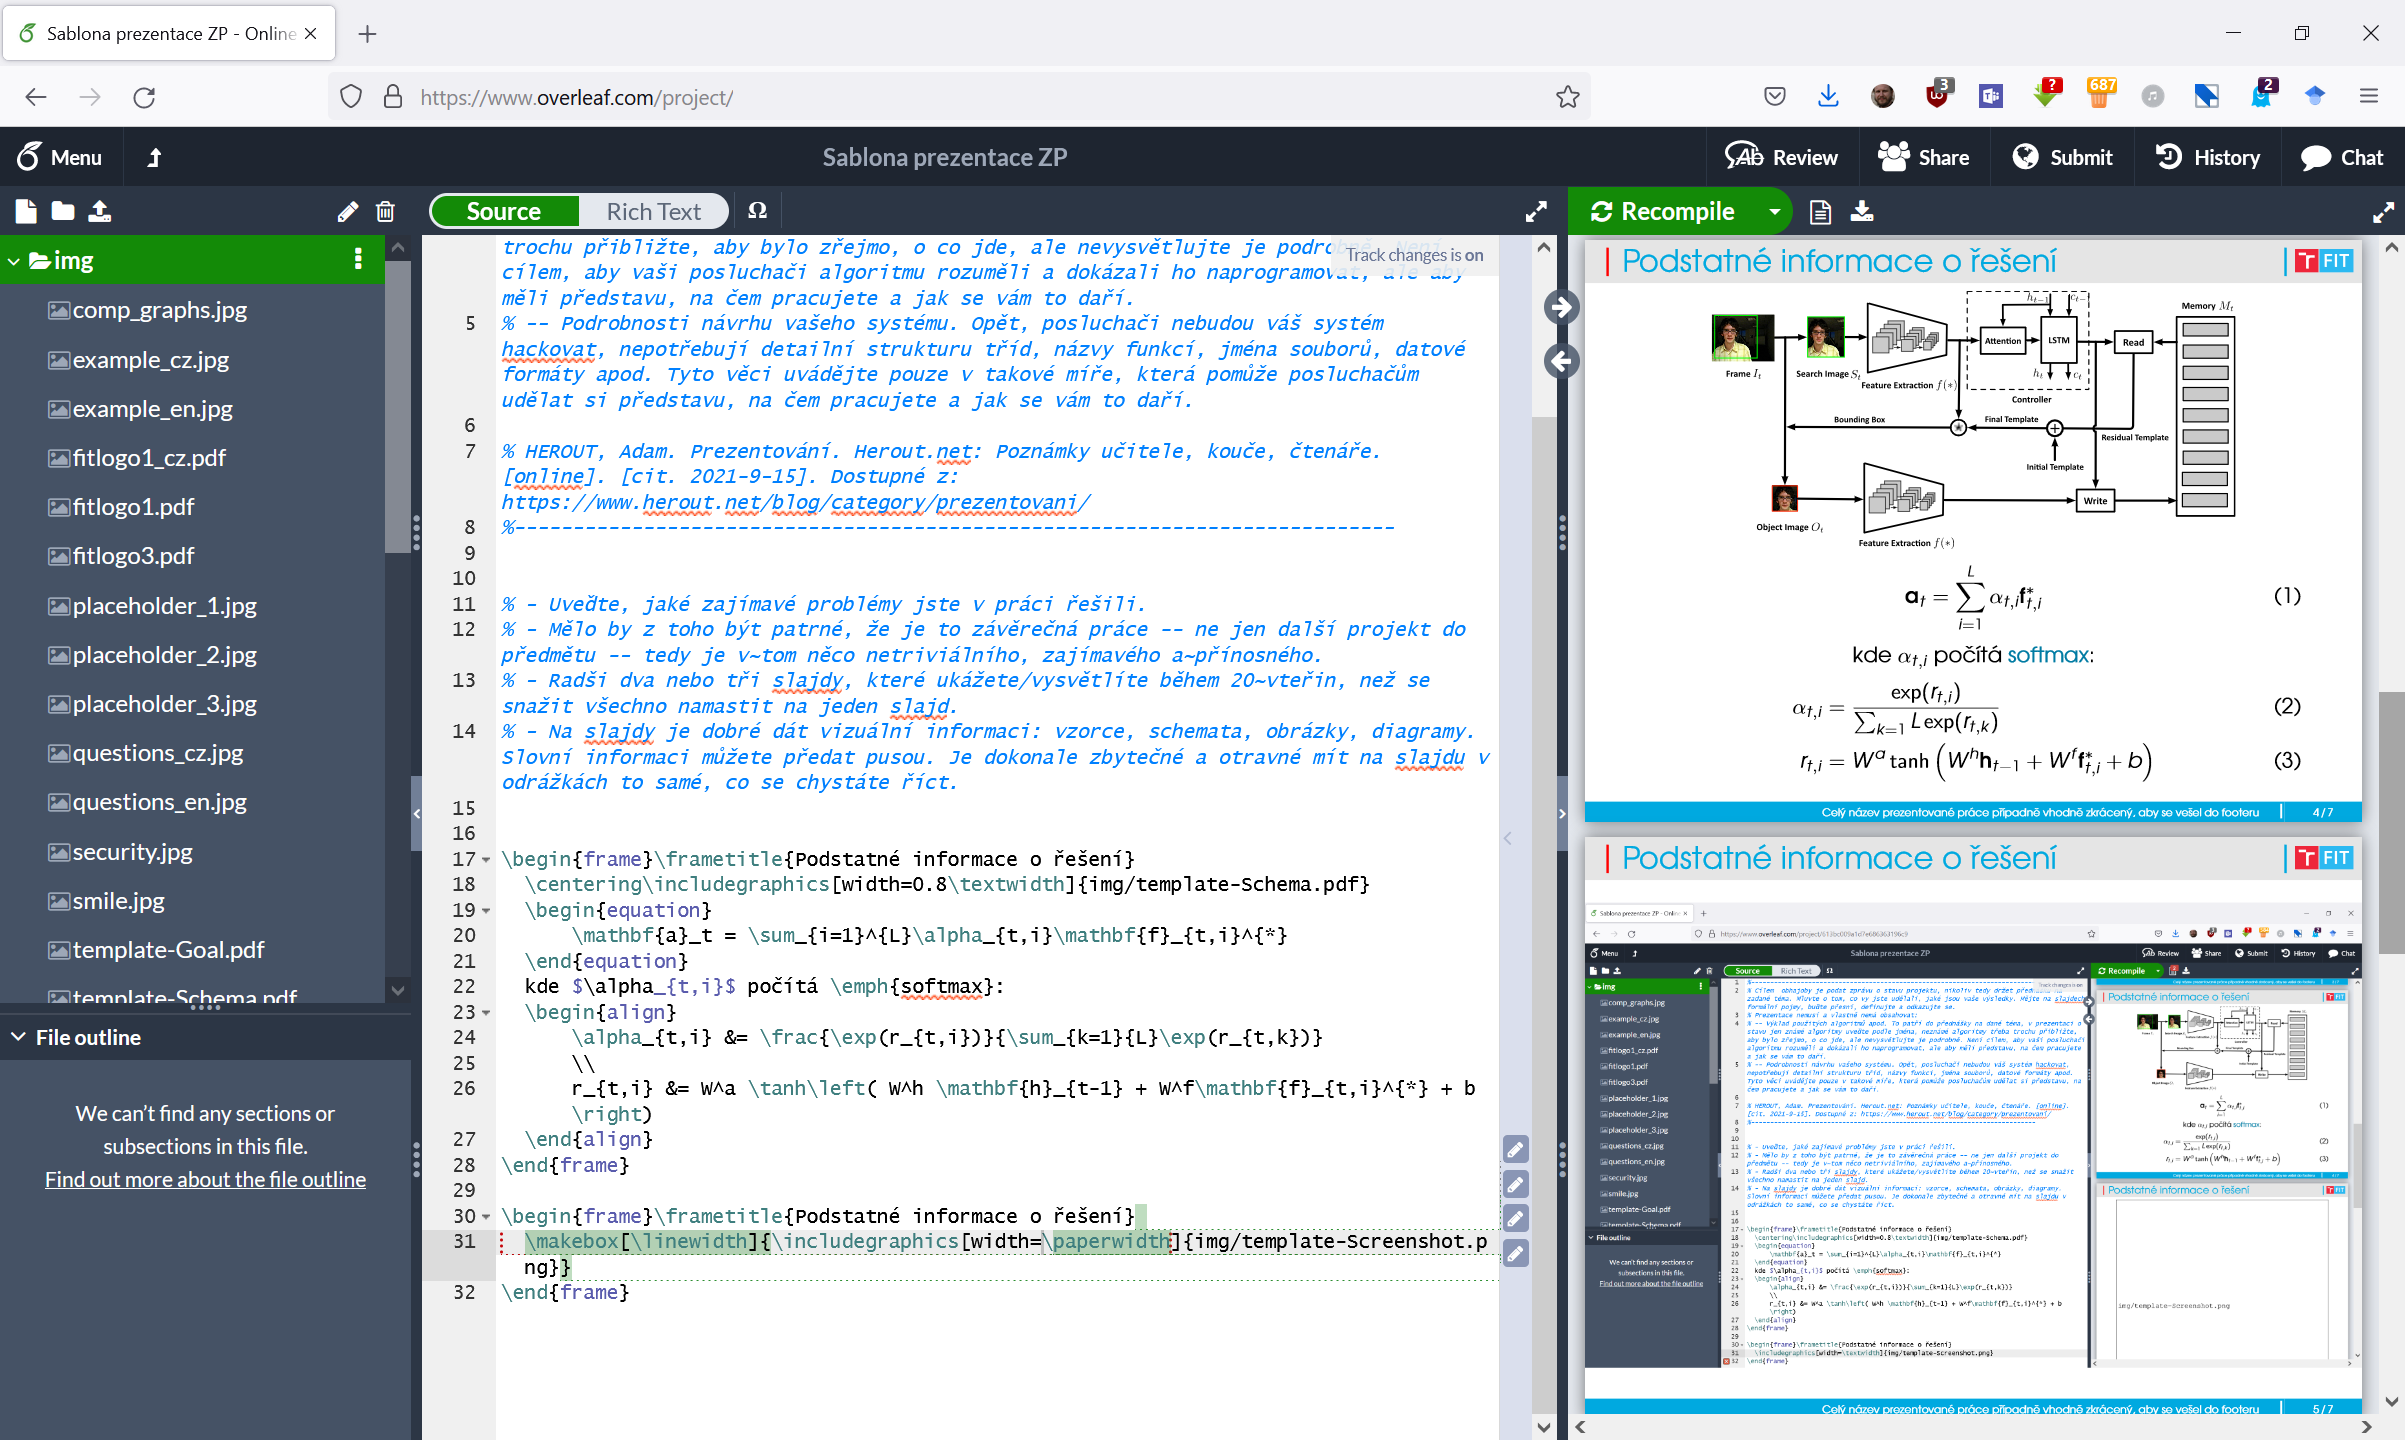
\includegraphics[width=\paperwidth]{img/template-Screenshot.png}}
    \end{frame}

    \begin{frame}
        \frametitle{Výsledky práce}
        \begin{columns}
            \column{0.4\textwidth}
            \begin{itemize}
                \item Co se \emph{podařilo}
                \item Vytvořená datová sada: \emph{105\,k} záznamů
                \item Úspěšnost: \emph{103\,\%}
            \end{itemize}

            \column{0.6\textwidth}
            \centering
            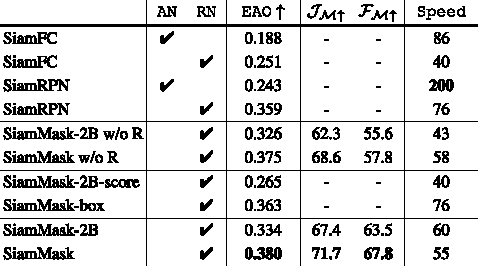
\includegraphics[width=0.8\textwidth]{img/template-ResultsTable.pdf}

            \bigskip
            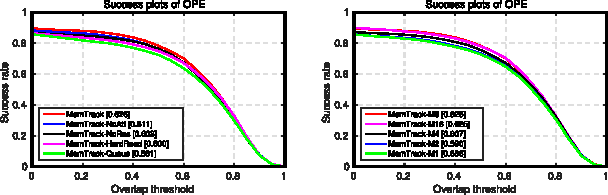
\includegraphics[width=\textwidth]{img/template-ResultsPlot.pdf}

        \end{columns}
    \end{frame}

    \begin{frame}
        \frametitle{Děkuji za pozornost!}
        \centering
        \makebox[\textwidth]{
            \begin{tikzpicture}
                \node (screenshot)
                {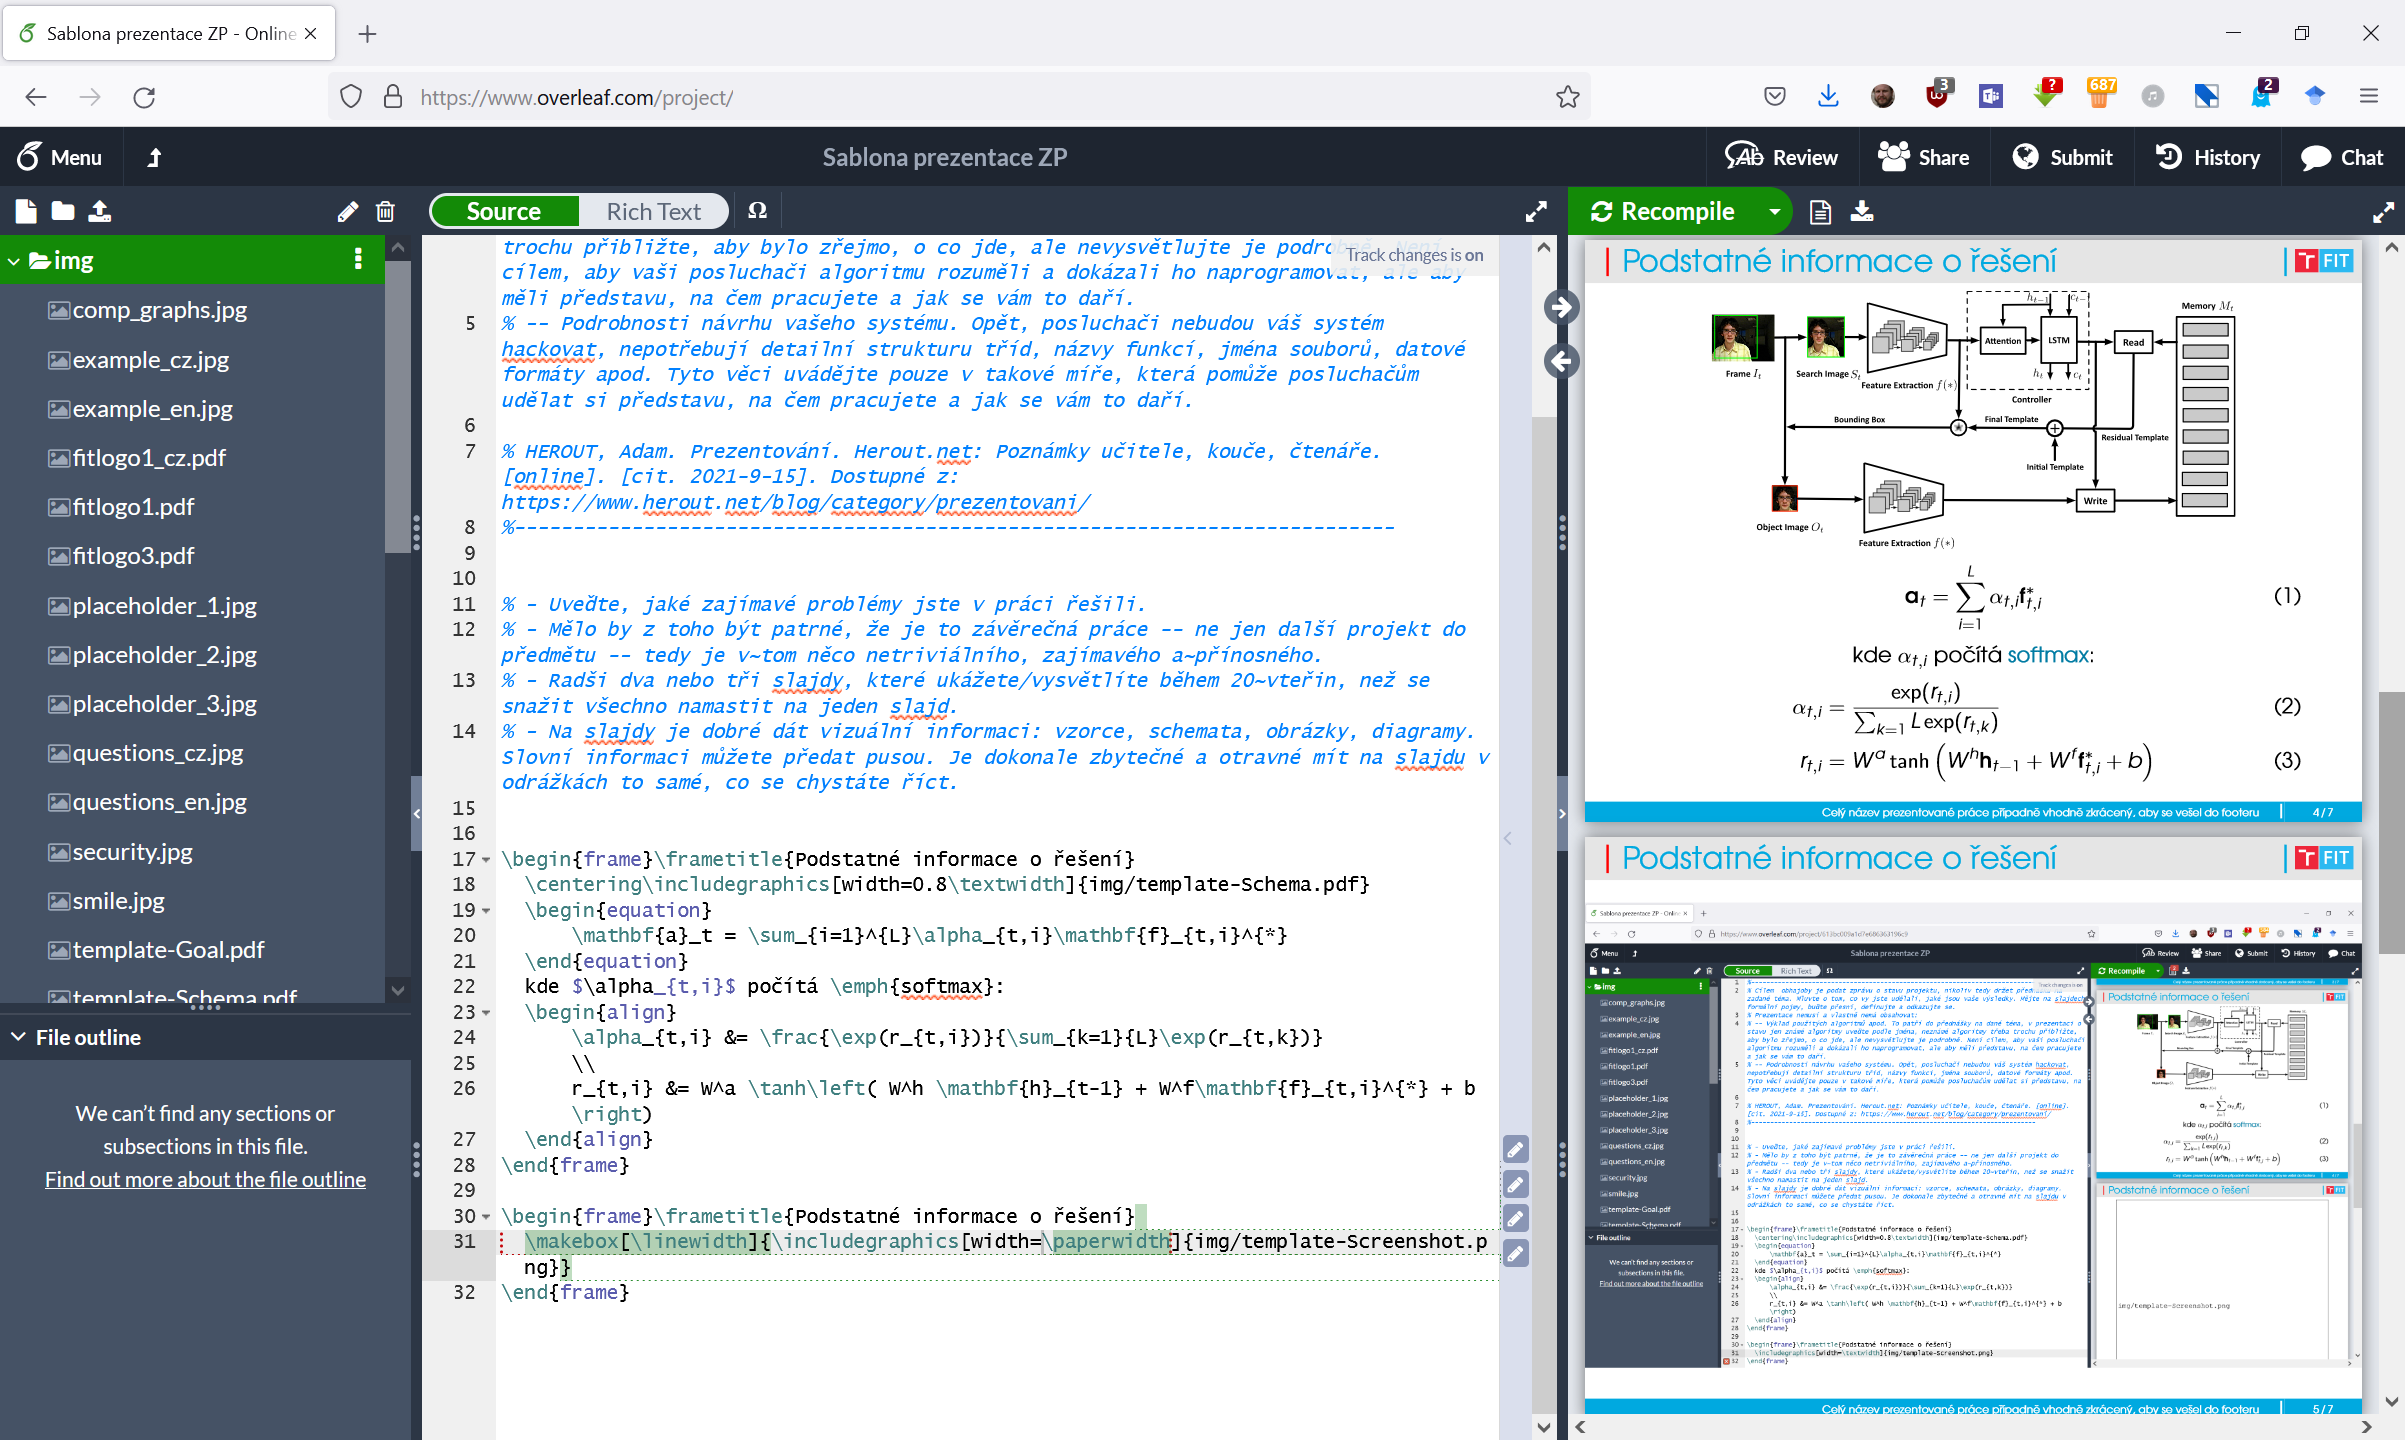
\includegraphics[width=0.6\paperwidth]{img/template-Screenshot.png}};
                \node (schema) at (screenshot.south east) [xshift=5em] [yshift=2.5ex]
                {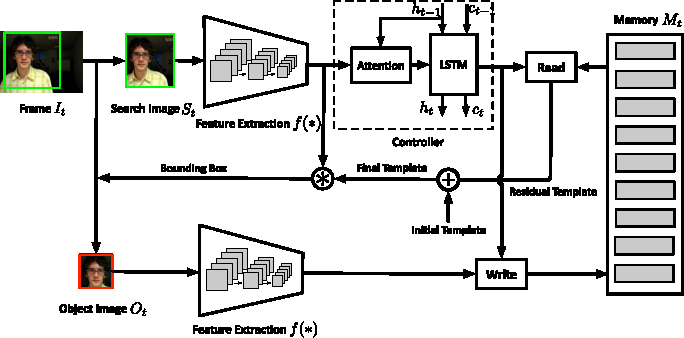
\includegraphics[width=0.45\paperwidth]{img/template-Schema.pdf}};
                \node (goal) at (screenshot.north east) [xshift=4em] [yshift=2ex]
                {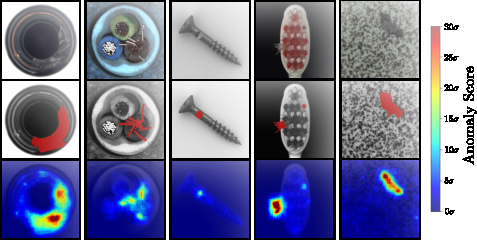
\includegraphics[width=0.5\paperwidth]{img/template-Goal.pdf}};
            \end{tikzpicture}
        }
    \end{frame}
\end{document}
